%===================================== CHAPTER 6 Design and architecture =================================

\chapter{Design and architecture}

To get a brief overview of the complete product and its required parts, the design and architecture are presented in this chapter. This is not meant to give a complete understanding of the system, but rather an overview on how the different parts of the product work together to give a pleasant user experience.

\section{Architecture}

The overall architectural design of the system was made to achieve a rough mapping of what needed to be done in terms of actual programming. The architecture focuses heavily on interactions between the different instances of the systems without going into the specific details on how this is done. To illustrate the architecture, two different views were created. One showing only the components, and the other showing the processes in the different components. The overall system structure can be seen in \textbf{Figure \ref{Fig:system_structure}}, this shows the four different components and how they interact. As shown in this diagram, the system is created as a client-server model, where the mobile application constitutes the client, which communicates with the PHP back-end server. The server is connected to a database, and Digitalt fortalt provides an API to retrieve stories from.\newline

\begin{figure}[h!]
	\centering
	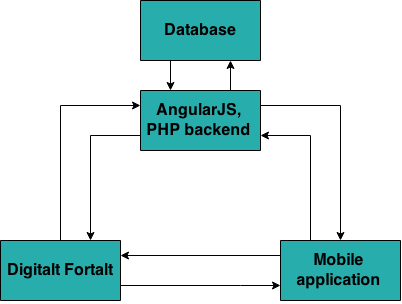
\includegraphics[width=0.45\textwidth]{fig/system_structure}
	\caption{Diagram of the overall system structure for this project.}
	\label{Fig:system_structure}
\end{figure}

\textbf{Figure \ref{Fig:architecture}} shows a diagram presenting the architecture for the application. As seen in the legend, the square boxes represent individual components or processes. The boxes with oval corners represent compound processes or larger parts. These are mainly shown because they give an overview of which processes belong to and will be performed by which part of the system. Double lined boxes are external sources which provide an API. Lastly, arrows indicate information flow.\newline

\begin{figure}[h!]
	\begin{center}
		\advance\leftskip-3cm
		\advance\rightskip-3cm
		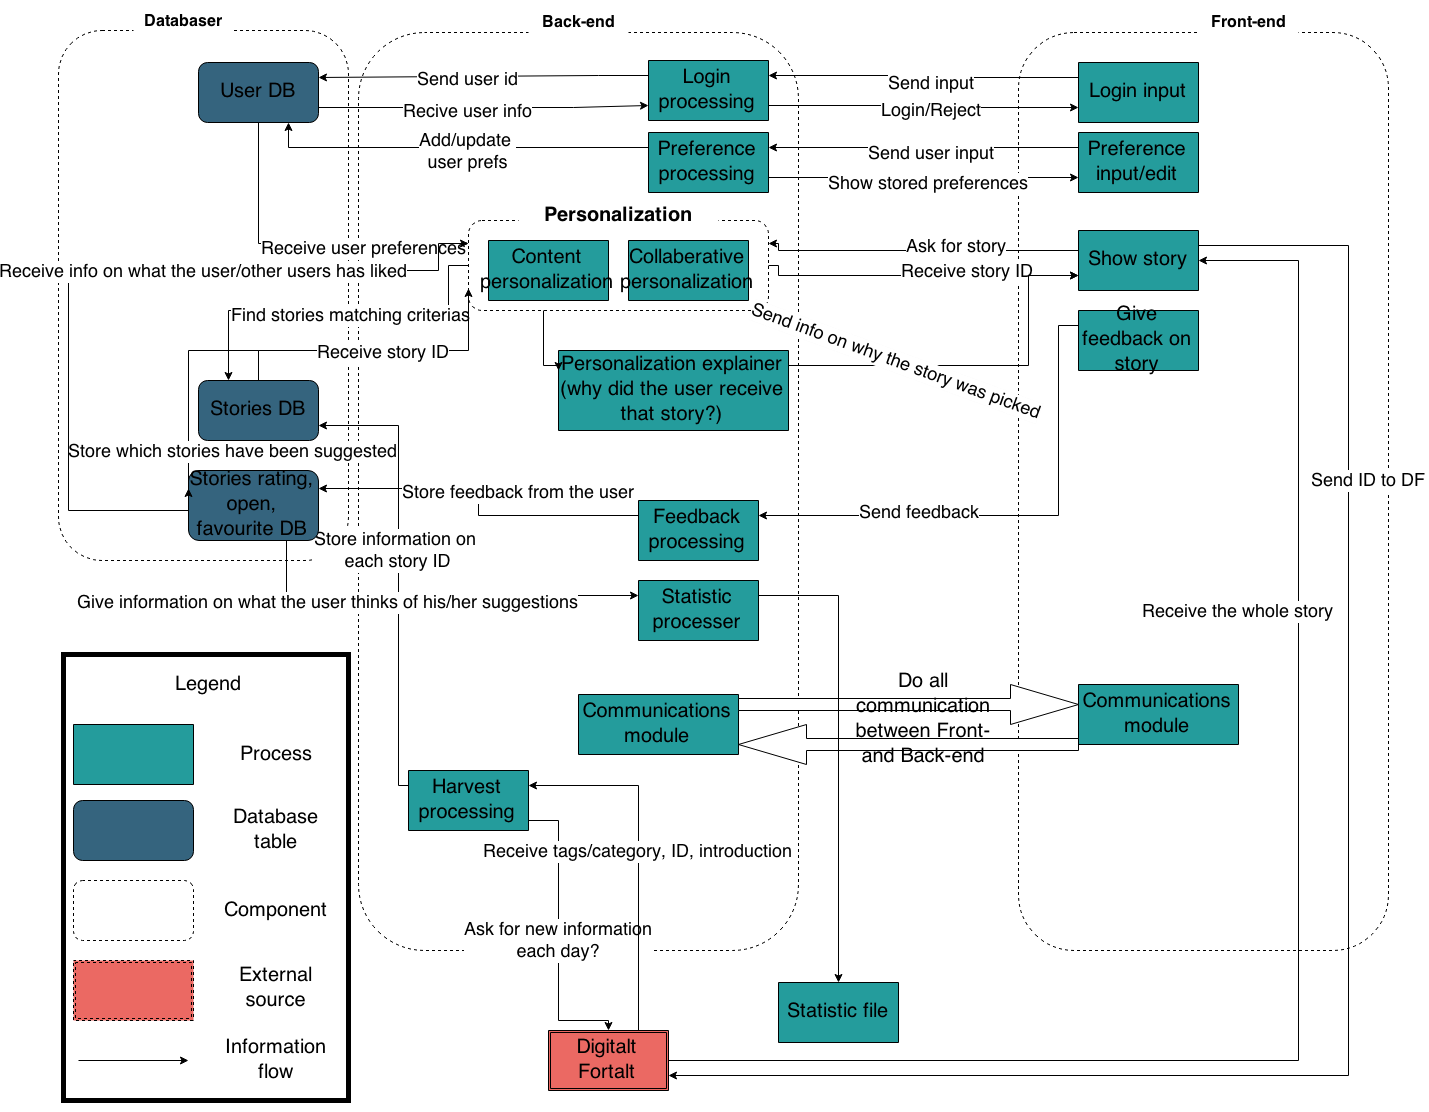
\includegraphics[keepaspectratio=true,scale=0.4]{fig/architecture}
		\caption{Diagram of the architecture for this project.}
		\label{Fig:architecture}
	\end{center}
\end{figure}

As seen in \textbf{Figure \ref{Fig:architecture}} the application structure is divided into three components; database, back-end and front-end. The front-end component is responsible for displaying information to the user. It also handles user input, which it conveys to back-end for processing (see \textbf{Section \ref{subsec:frontend-backend_communication}}). How front-end is built up and what is displayed to user can be found in \textbf{Sections \ref{sec:frontend_structure}} and \textbf{Sections \ref{sec:design_user-interface}}, respectively. The back-end section is responsible for handling requests from front-end, returning information to front-end and for harvesting the stories stored in the database from Digitalt fortalt. \textbf{Section \ref{sec:backend_overview}} describes the back-end structure. The database component stores all the persistent information related to users and stories. The database is described in \textbf{Section \ref{sec:database_design}}.   \newline


It is a difficult task to model a whole system in an accurate way, and while the architecture diagram gives an overview, it can not give much insight into the complexity of each process. This is further complicated by the fact that in the startup phase of the project there are a great number of unknowns. Both complexity and requirements are subject to change. As such, the diagram should only be used as a guide for understanding the composition of the complete system.

\section{Front-end structure}
\label{sec:frontend_structure}
The front-end of the application was designed by using Ionic and AngularJS and this section will describe how a system made in AngularJS is structured.\newline

AngularJS provides templates to create systems based on a Model-View-Controller (MVC) architecture, and also provides a variety of components to assist in making the programming more effective and speeding up the application. It is essentially another layer of abstraction above writing regular JavaScript. These are some of the main concepts that are used to create an Angular application:

\begin{description}
	\item[Model] \hfill \\ 
	Manages all the data that can be interacted with by the user. The model also keeps the views up to date and can be manipulated by controllers.
	
	\item[View] \hfill \\ 
	The interfaces that the user can see. This means some form of visual representation of the model.
	
	\item[Controller] \hfill \\ 
	The logic and behavior of the views. The controllers also make changes to the model.
	
	\item[Directive] \hfill \\ 
	Special functionality applied to the DOM elements, you can create your own directives as well as use the numerous ones provided by AngularJS itself. In "Vettu hva?", several of these were used, such as directives that call on some function when DOM elements are clicked on, or directives that show or hide parts of the DOM based on some condition.
	
	\item[Module] \hfill \\ 
	A module encapsulates a part of the application. Instead of having a single "main" function that holds the application together, Angular applications normally have multiple modules that work together. The benefit of this is that the application is decomposed into logical parts that can be reused, loaded, and tested in any order. In "Vettu hva?", each controller is its own module. The part of the program that communicates with the back-end is also encapsulated in a module. Furthermore, there is a module that starts up the application and binds together views and controller into different states.
	
	\item[Scope] \hfill \\ 
	The scope contains all the elements that the application currently has access to. It can be viewed as a container that stores the current model, and so if a controller or directive is going to modify or access the model, this has to be done by using the scope.
	
	\item[Service] \hfill \\ 
	A service contains "global" logic that is accessible to the entire application. In "Vettu hva?", this is used in the module that contains the communication with the back-end. This module has three different services, which respectively gives the application access to user data, story data, and requests from front-end to back-end.
\end{description}

\section{User interface}
\label{sec:design_user-interface}

\begin{figure}[h!]
	\centering
	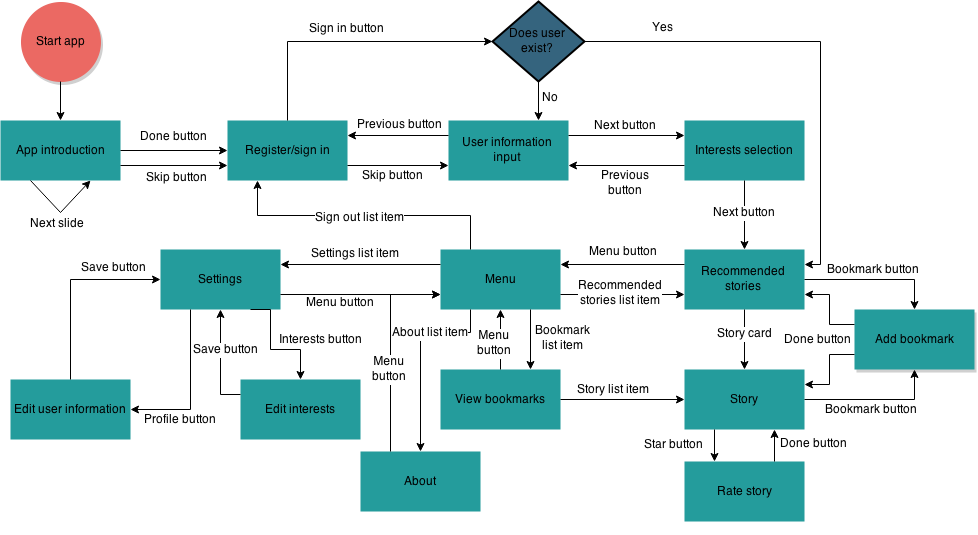
\includegraphics[width=\textwidth]{fig/flow_diagram}
	\caption{Diagram of the flow between views in the user interface.}
	\label{Fig:flow_diagram}
\end{figure}

It was very important to the customer that the application should be easy to use (\textbf{Section \ref{sec:non-functional_requirements}}). The elements added to the user interface were thus only things that were absolutely needed in order to satisfy the customer's requirements. The customer also wanted it to "feel native". As it would be very time consuming to make two very different designs for Android and iOS, the design of the app was made quite different typical Android or iOS. This way it would not look out of place on either platform, and it would not be dated as easily when new operative system versions come out. For example, the hamburger menu pattern can be found on both platforms. This also made the interface simpler as the functions that are not used as often can be out of sight. It helped the focus on the main function, exploring stories.\newline

The usability of an application is not just about the individual views, it is also about the structure and flow of the app. \textbf{Figure \ref{Fig:flow_diagram}} explains the overall flow between all the different views in the application. The green boxes represent views, while the white ones represent modals placed on top of the view the user came from. The text of the arrows explain what the user clicked in the view the arrow comes from, and the arrow points to which view this action leads to.  The functionality of the more complex views will then be explained in further detail. The rest of the views can be found in the user manual (\textbf{Appendix \ref{app:user_manual}}). 



\begin{description}
	
	\item[Recommendation view] \hfill \\ 
	This view displays the stories that should be the most relevant to the user. The user can browse them by swiping through them or by clicking the left and right arrows. When tapping on a card the detailed view of the story will be displayed. The bookmark icon in the top bar opens a modal for adding a bookmark. 
	
	\begin{figure}[h!]
		\centering
		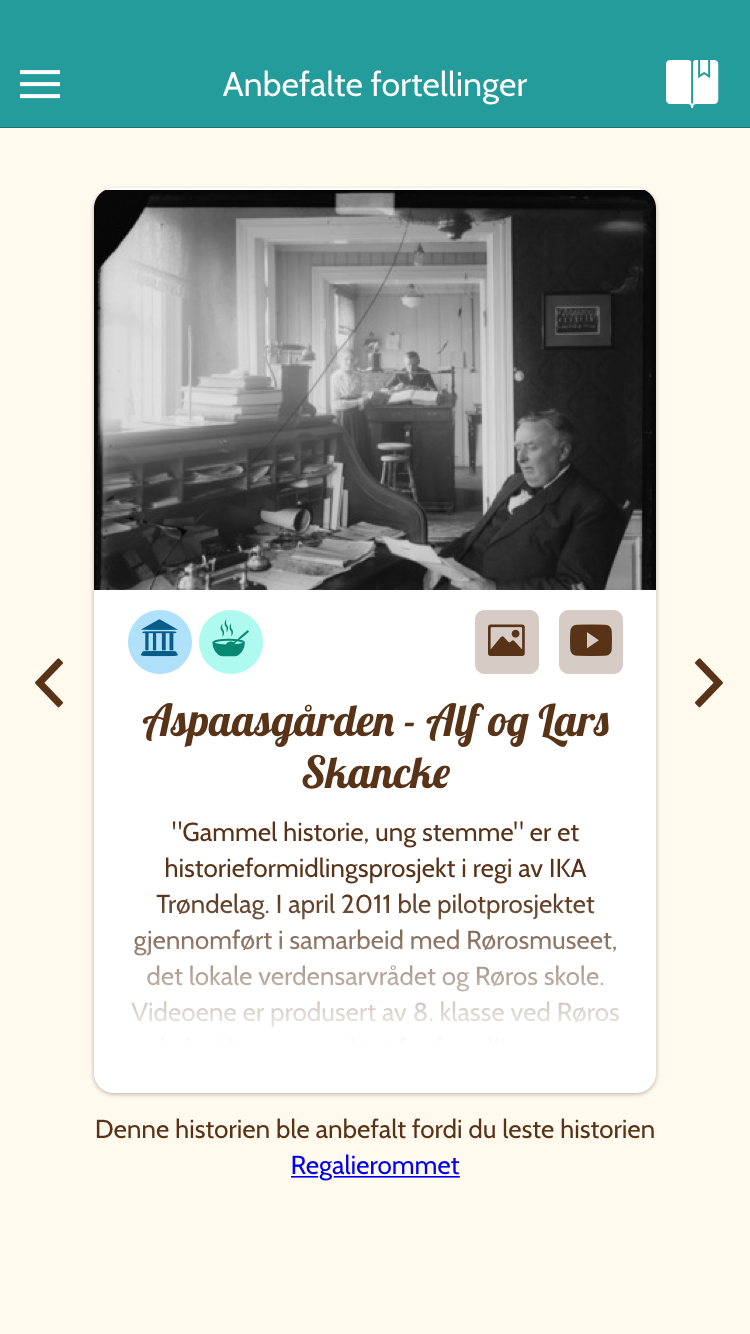
\includegraphics[width=0.4\textwidth]{fig/screenshot_recommendations}
		\caption{Recommendation view}
		\label{Fig:recommendation_view}
	\end{figure}
	
	\item[Story view] \hfill \\
	This view displays the chosen story in detail. There is a box which displays the media files associated with the story. The tabs above it will depend on which media types the story contains. Videos will be displayed by default if there are any, as they can be a major component of the story which should not be hidden in another tab. When tapping on a video or image it will be displayed in fullscreen mode. The user can give feedback on the story either by tapping the stars on the bottom part of the view, or by tapping the star icon in the top bar which will open up a modal. The modal will ask the user to rate the story, and the user can exit it by tapping “Ferdig” or by tapping outside of the modal. Tapping the bookmark icon will make the same modal as in the recommendation view appear. 

\end{description}

\begin{figure}[h!]
	\ContinuedFloat
	\centering
	
\includegraphics[width=0.4\textwidth]{fig/screenshot_story}
	\caption{Story view}
	\label{Fig:story_view}
\end{figure}

\section{Front-end - back-end communication}
\label{subsec:frontend-backend_communication}

Communication between front-end and back-end was handled using HTTP post requests.
AngularJS \$http is a core service for reading data from remote servers, which is called every time the application needs to add, retrieve, update or delete data. When an HTTP request is made, four fields are set: method, headers, URL and data. The method field determines the HTTP request method, which in this application is set to post, and the headers field sets the content type to JSON. The URL is the location of the remote server script that handles HTTP requests. In the data field the action to be executed is specified, in addition to any data needed to perform the desired action.\newline

Each HTTP request is managed by the same back-end PHP script. This script decodes the HTTP request, determines which action to perform and executes it. When the script has finished executing, a JSON response is returned to front-end with the desired data. "Get story" is an example of a request. When a user wishes to read a story front-end sends the JSON formatted paramaters userId, storyId and request type, in addition to the previously mentioned fields, as an HTTP request to back-end. Back-end retrieves story information from the database and Digitalt fortalt, which is then returned as a JSON formatted response to front-end. Other request examples are "Add user", "Edit user" and "Get recommended stories".

\section{Back-end overview}
\label{sec:backend_overview}

The back-end design is divided into five sections, such that each section addresses a separate concern. A concern is a set of information that affects the code of the application. The value of such a separation is that it simplifies the development and maintenance of the application code. By splitting the code into separate parts the system is more logically structured, and cleaner code is achieved. The result is as an example that SQL related code is maintained by one part of the system, while HTTP processing is executed by another. Below is a description of the different back-end sections.

\begin{description}
	\item[Models] \hfill \\
	Consisting of the classes storyModel, userModel and preferenceValue. The models are used to temporarily hold information about a story, a user and a user's preference value for a story to be utilized by other files. Information is either retrieved from the database, sent from front-end, harvested from Digitalt museum's API or a combination of these. These models also contain formatting methods, which makes it possible to return story or user information to front-end.
	
	\item[Database] \hfill \\
	This section contains the classes dbStory, dbUser, dbHelper and harvesting. The db classes are responsible for accessing the database. dbStory contains methods for adding or retrieving story related information from the database and dbUser is responsible for user related information. dbHelper consists of more general methods and is the class which establishes a connection with the database. The harvesting script is responsible for collecting all database stories from Digitalt museums API and adding stories to or updating stories in the database (see \textbf{Section \ref{sec:harvesting}}).
	
	\item[Personalization] \hfill \\
	Consisting of the classes computePreferences and runRecommender. This section computes preference values for each Digitalt fortalt story in the database for each user. runRecommender is also responsible for initializing the Mahout recommendation engine when a user's preference values have been calculated.
	
	\item[Recommender] \hfill \\
	This section consists of the Java code and recommender.jar file which make up the Mahout recommender (see \textbf{Section \ref{sec:personalization_how}}).
	
	\item[Requests] \hfill \\
	Contains the controller script, which receives and handles front-end HTTP requests and returns JSON responses (see \textbf{Section \ref{subsec:frontend-backend_communication}}).
	
\end{description}

\textbf{Figure \ref{Fig:overall_backend}} depicts the different back-end classes introduced in the previous paragraphs and give an overview of their dependencies.

\begin{figure}[h!]
	\centering
	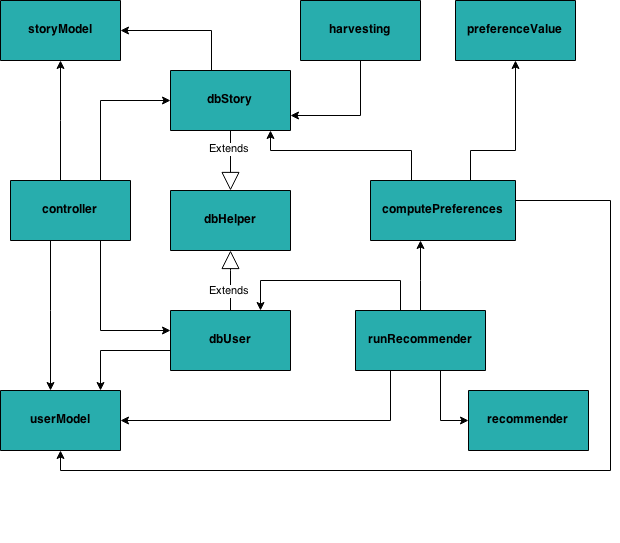
\includegraphics[keepaspectratio=true,scale=0.6]{fig/overall_backend}
	\caption{Class diagram of the overall back-end structure}
	\label{Fig:overall_backend}
\end{figure}

\section{Category mapping} 
\label{sec:categorymapping}

There are 31 subcategories present at Digitalt fortalt. Each story can have 0 to 31 subcategories attached to it. To achieve content-based filtering the user has to select some categories of interest. To make it easier for the user, these subcategories are divided into nine main interest categories. Some of these categories were already predefined in a TAG CLOUD document provided by the customer, while the rest was decided in discussions with the customer. The subcategories were put into the category interest field that fit them best, with some subcategories being in several category interests. In \textbf{Table \ref{Tab:categorymapping}} this mapping is illustrated. It is obvious that some category interests will have more stories, and some subcategories such as history contain more stories than most others. It was intended to create nine category interests that contain roughly the same amount of stories. However, when a subset of stories was chosen this intention did not hold true as can be seen in chapter \textbf{Section \ref{sec:harvesting}}. Furthermore, the category interests needed to be distinct while still encompassing all the subcategories. 

\begin{table}[!h]
	\begin{center}
		\caption{Category mapping performed to facilitate, and simplify content-based filtering. Each subcategory is assigned to one or more category interests.}
		\label{Tab:categorymapping}
		\begin{tabular}{ | p{5cm} | p{12cm}|}
			\hline
			\textbf{Archeology} & Arkeologi og forminne \\ \hline
			\textbf{Architecture} & Arkitektur \\ \hline
			\textbf{Art and design} & Bildekunst, dans, design og formgjeving, film, fotografi, media, teater \\ \hline
			\textbf{History} & Historie, historie og geografi, kulturminne, sjøfart og kystkultur, språkhistorie \\ \hline
			\textbf{Local traditions and food} & Bunader og folkedrakter, dans, fiske og fiskeindustri, fleirkultur og minoritetar, Hordaland, kultur og samfunn, kulturminne, musikk, Rallarvegen, samer, sjøfart og kystkultur, språk, tradisjons- mat og drikke \\ \hline
			\textbf{Literature } & Litteratur, teikneseriar \\ \hline
			\textbf{Music} & Musikk \\ \hline
			\textbf{Nature and adventure} & Fiske og fiskeindustri, naturhistorie, sport og friluftsliv \\ \hline
			\textbf{Science and technology} & Fiske og fiskeindustri, fotografi, "kjøretøy, bil og motor, veitransport", media, "natur, teknikk og næring", "teknikk, industri og bergverk", skip- og båtbygging \\ \hline
		\end{tabular}
	\end{center}
\end{table}


\section{Digitalt museum's API and harvesting}
\label{sec:harvesting}

The content of the stories displayed in the application was collected from Digitalt fortalt. At the request of the customer the stories collected are limited to the areas Nord-Trøndelag and Sør-Trøndelag. The reason for this was that it would increase the likelihood of users reading similar stories, and thus make it easier to evaluate the personalization. The API \cite{digitaltMuseum} used to retrieve stories belongs to Digitalt museum. This API enables search through data from Digitalt museum, displaying pictures, and provides access to an XML representation of available objects. Digitalt fortalt is established on the same technical platform as Digitalt museum \cite{HM2}. This makes the integration better between the two and the remaining services in Norvegiana. Norvegiana is a data model, database and a web service with the purpose of making cultural heritage information more accessible \cite{HM3}. Example services available in Norvegiana are Digitalt museum, Digitalt fortalt, Arkivportalen and Musikkarkiv.\newline 

Some info, such as the categories for each story, are harvested and stored in the database. This is mainly to facilitate personalization. The actual story and the related media are fetched from Digitalt fortalt at the request of a specific story from front-end. At the time of writing the number of harvested stories is 169. This may vary as the harvesting is done each day. The stories are distributed unevenly over the nine categories; both the history and local traditions categories have over one hundred stories connected to them, while the literature category only have two stories connected to it. Media formats distribution also varies, with only fifteen stories having sound and both picture and video included in over one hundred stories.  

\section{Personalization}
\label{sec:personalization_how}

Users receive recommended stories by means of content-based and collaborative filtering, as described in \textbf{Section \ref{sec:personalization_algorithms}}. The system gathers information about the stories and the users, and feeds this information into the recommender engine Mahout which produces a list of recommendations for the specified user. The details of Mahouts inner workings will not be presented here. What will be described is how the input data delivered to Mahout is gathered and produced by our application, what methods of Mahout is used and when they are used, and how the resulting list of recommendations is dealt with.\newline

Both content-based and collaborative filtering rely on giving a numerical value that express how much a user likes a story. We call this a preference value. In our application this value is computed by combining several measures representing different types of user feedback. These are: the rating a user have given to a story, the categories the user has expressed an interest in, the number of times a story has been recommended to the user, the number of times the story has been opened and the number of times a story has been put in the to-be-read list. Weights are assigned to the measures to differentiate between what impact they should have on the preference value. Rating is considered the most important user feedback, since this value is given to a story by direct user action. The other measures are either less connected to a specific story or more intangible. When computing recommendations, preference values for all stories for the user in question are calculated first.\newline

Each time Mahout is run, up to ten recommendations are inserted in the database. How these are chosen depends on a number of factors. Since a requirement from the customer was to include false recommendations, one of the recommendations is always picked from the lower parts of the recommendation rankings. The other stories are picked from the top of the rankings. Depending on two factors some top recommendations may be skipped for a given run. The first of these factors is that rated stories are not recommended again to the user (only an issue for content-based filtering). The other one is whether the list of recommendations should be added to the existing list of recommendations browsed by the user in the recommendation view or not. When adding to the existing list, recommendations should not be repeated. Adding to list happens when the user draw near the end of the current list of recommendations in the recommendation view, while new recommendations are computed when the user rates a story, changes its category interests or leaves the application (to make sure the recommendations are fresh next time the user enters the application).\newline

Mahout uses a data model and a similarity model to compute recommendations. The data model is a collection of triplets, where each triplet consists of a user ID, a story ID and a preference value. The selection of which preference values to include is different in content-based and collaborative filtering. The similarity model is also different for content-based and collaborative filtering. A description of these differences follows in the subsequent sections.    

\subsection{Content-based filtering}

When doing content-based filtering, the input data model consists of a collection of all the preference values for the user we are making recommendations for. This means that the size of the model will be equal to the number of stories harvested from Digitalt fortalt. To make recommendations Mahout also need measures describing how similar stories are. Similarities between stories are computed based on the subcategories found in the second column in \textbf{Table \ref{Tab:categorymapping}} using the cosine similarity formula: 

\begin{equation}
similarity = \frac{\vec{x}\cdot\vec{y}}{||\vec{x}||\cdot||\vec{y}||}
\end{equation}

The dot product in the numerator is in our system equivalent to the number of common subcategories for two stories, while the denominator is the product of the square roots of the number of subcategories for each of the two stories. If two stories have exactly the same subcategories the similarity value will be 1, and if they do not share any subcategory the value will be 0. \newline

These similarities are computed and put in a comma-separated values (CSV) file after the harvesting is done. This file is read before the recommendations are computed and the similarity values are put in the appropriate Mahout objects. Mahout then uses the data model and the similarity model with similarity values for all possible pairs of stories to produce a ranked list of recommendations. This list is enhanced with an explanation of why a story was recommended, using a Mahout method that returns the stories most influential for a given recommendation.


\subsection{Collaborative filtering}

Collaborative filtering uses a data model with multiple users. Only the stories a user has rated will be included in the data model since this is the most precise user feedback. In our application collaborative filtering is done by combining two different methods provided by Mahout, namely item-based recommendation and user-based recommendation. The item-based approach creates a similarity model based on similarity between items in the data model using a logarithmic Likelihood function, while the user-based approach creates a similarity model based on similarity between users in the data model using Pearson correlation. To prevent dissimilar users from affecting the recommendations in the user-based approach, a threshold value for the similarity is set. The two lists of recommendations are produced and then merged, assuming both have content to get one list of ranked recommendations. If only one of the lists has content then the predicted rating for the story is used to decide what story to serve next.\newline

As was noted in \textbf{Section \ref{sec:personalization_algorithms}} collaborative filtering requires a large amount of data to make recommendations. Since only rated stories are included, collaborative filtering cannot be run when a new user starts using the application as the user will not be part of the data model. The criteria for using collaborative filtering needed to be met is that the user has rated at least ten stories which at least ten other users also have rated. In the event of too few collaborative story recommendations content-based filtering is used. 

\section{Database design}
\label{sec:database_design}

The database was designed with the goal of facilitating the recommendation of stories to users. The data model underpinning the database is visualized in the ER-diagram in \textbf{Figure \ref{Fig:er_diagram}}. User and story are the central entities in this diagram, since the goal of the application is to connect users to stories. Both of these entities has a number of attributes describing the entity. The central relationship in the diagram is the recommendation-relationship, where a user and a story is connected. This connection is described by some additional attributes, such as rating, tag (which is the same as a bookmark) and state. \newline

\begin{figure}[h!]
	\centering
	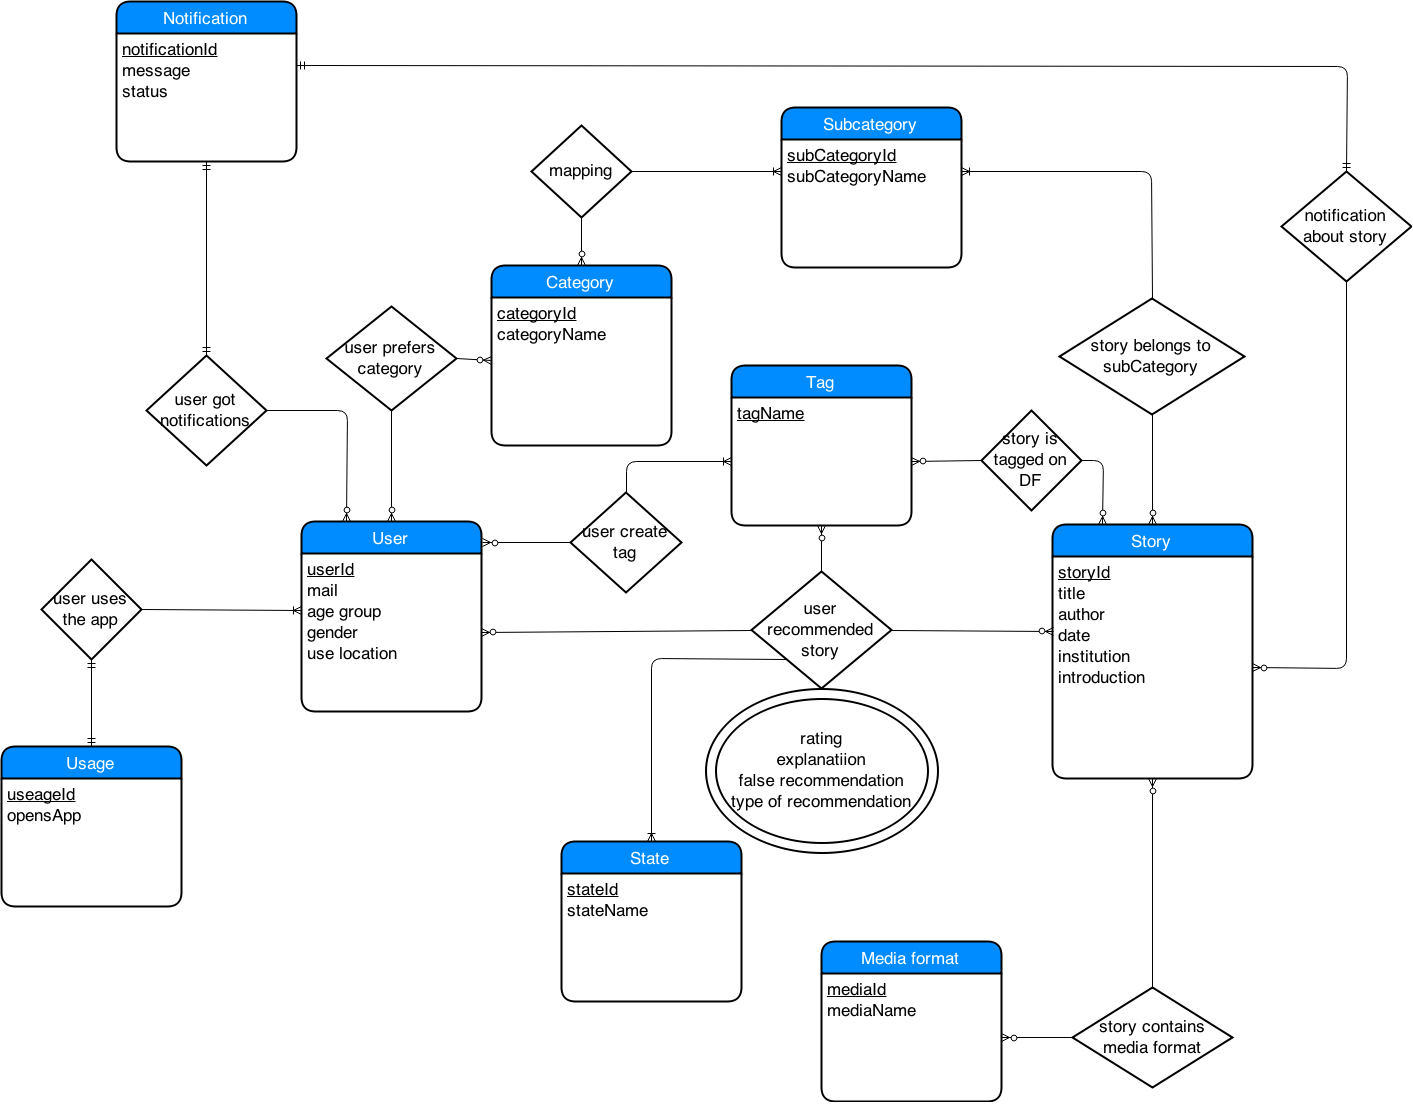
\includegraphics[width=\textwidth]{fig/er_diagram}
	\caption{ER-diagram showing the data model}
	\label{Fig:er_diagram}
\end{figure}

To make the right connections between user and story, some attributes describing the user and the stories are necessary to store in the database. For instance, in order to make recommendations based on nine predefined categories, every story is mapped from subcategories gathered from Digitalt fortalt to one or more of the nine categories (see \textbf{Section \ref{sec:categorymapping}}). A user is connected to one or more of these categories by the setting of personal preferences. The changing state of recommended stories is also recorded, partially to make better recommendations and partially for research purposes. \newline

As described in \textbf{Section \ref{subsec:summary_functional_requirements}} a requirement for the project was to provide some research data to the customer. To do this some data about the use of the application is stored, including registering what actions are taken during a user session with regards to a story. The state entity records changes in the state of a story for a specific user. The state diagram in \textbf{Figure \ref{Fig:state_diagram}} shows the states a story can have and the possible transitions between them. There are four states in our system (recommended, read, to-be-read and rated), all of which can be recorded multiple times for a story for a given user. The labels on the arrows between states are the events that trigger the transition from one state to another, with one exception: the "Story not rated"-label (marked with a border around the text). This is a boolean condition which must evaluate to true to enable the transition. For our system, this means that a story can be recommended again after it has been opened (read) or bookmarked with "Les senere" (to-be-read), but only if the story has not been rated at any point. Another point to emphasize is that a story has no state in the system before it has been "Viewed" (seen in the state diagram as the initial transition from the solid circle which represent the start point). A story is "Viewed" when the user sees the story in the recommendation view at front-end. This means that the only way a user can experience a story is to be recommended the story. 

\begin{figure}[h!]
	\centering
	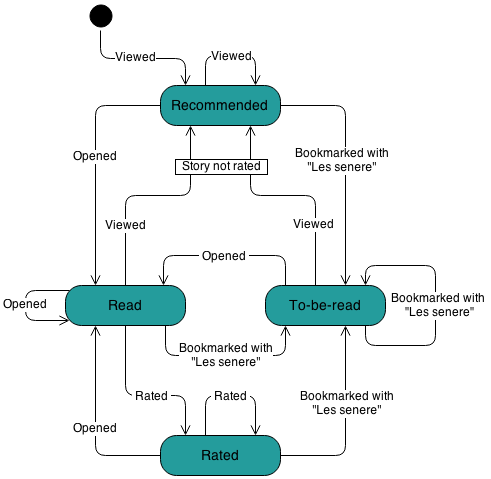
\includegraphics[height=11cm]{fig/state_diagram}
	\caption{State diagram showing states and transitions for a story for one user}
	\label{Fig:state_diagram}
\end{figure}


\section{Docker}
\label{subsec:docker}

Docker \cite{EHW2} was made to help automation of application deployment. This happens by providing a virtual operating-system-level abstraction. This means that on a server, it is possible to run several virtual operating systems called docker images, which can easily be deployed to another server. This is beneficial for software development, because it means it is easy to setup identical back-ends at different locations. The customer used this on their servers, which made using it during development a good choice as well. A benefit of using docker is that it can directly access repositories on Git. This means that the latest revision is guaranteed to run when starting the back-end. However, there are also drawbacks. It is not easy to update files within the docker image currently running without rebuilding it. This means that to update a single line of code, the whole image needs to be rebuilt. Which means that while the newest revision is guaranteed to be running, any changes made to the application after the start of that docker image requires manually stopping, rebuilding, and restarting the docker image. \\

A docker image based on Ubuntu was used. In the Dockerfile, which is used to automate the deployment, all required dependencies were installed through Ubuntu's command line. A Linux, Apache, MySQL, and PHP (LAMP) stack and Java were the most critical dependencies. The setup of these tools was written to files which are downloaded from GitHub at runtime along with the back-end source files. After the Dockerfile is run an image is built and launched as wanted.


\cleardoublepage